\documentclass[12pt]{report}

\usepackage[a4paper, top=4cm, left=4cm, right=3cm, bottom=3cm]{geometry}

\usepackage{amsmath}
\usepackage{graphicx}
\usepackage{listings}

\title{Laporan Tugas Teori Bahasa Formal \& Otomata :\\ Implementasi DFA pada \textit{Marble Rolling Toy}}
\author{Turfa Auliarachman, 13515133}
\date{17 September 2016}

\lstset{showstringspaces=false}

\begin{document}
  \pagenumbering{gobble}
  \maketitle
  \newpage
  \pagenumbering{arabic}
  \tableofcontents
  \chapter{Deskripsi DFA Terkait}
  \section{Deskripsi Persoalan}
Terdapat sebuah \textit{marble rolling toy} seperti pada gambar berikut :
\begin{figure}[h!]
  \centering
  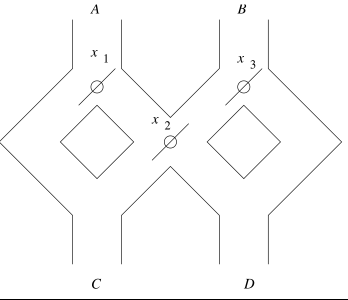
\includegraphics[width=250pt]{gambar.png}
  \caption{Ilustrasi \textit{Marble Rolling Toy}}
\end{figure}

\textit{Marble} akan digelindingkan dari A atau B. Ketika mengenai penghalang ($x_1, x_2, x_3$), \textit{marble} akan diarahkan sesuai penghalang tersebut. Lalu, penghalang yang dilalui \textit{marble} akan berganti arah. Jika \textit{marble} keluar di D, maka permainan dianggap berhasil. Mula-mula, semua penghalang menghadap ke kiri.

Permasalahan di atas ditranslasikan sebagai permasalahan DFA. Lalu, harus dibuat sebuah program dalam bahasa C atau Pascal yang memproses permasalahan DFA yang definisinya ada di sebuah file eksternal, lalu mengetes apakah string masukan pengguna diterima oleh DFA atau tidak. Program DFA itu akan digunakan untuk mengetes pada persoalan \textit{Marble Rolling Toy} apakah \textit{marble} terakhir masukan pengguna keluar di D atau tidak.

  \section{DFA}
\label{sec:DFA}
Translasi permasalahan \textit{Marble Rolling Toy} dalam notasi DFA :
\begin{equation*}
  A = (Q, \Sigma, \delta, q_0, F)
\end{equation*}
di mana
\begin{align*}
  \centering
  Q &= \{LLLC, RLLC, LRRC, LRLC, RRRC, LRLD, \\&RRLC, LLRD, RRLD, LLLD, RLRD, RLRC, RLLD\} \\
  \Sigma &= \{A, B\} \\
  q_0 &= LLLC \\
  F &= \{LRLD, LLRD, RRLD, LLLD, RLRD, RLLD\} \\
\end{align*}
dan $\delta$ dalam tabel berikut :
\begin{table}[h!]
  \centering
  \caption{Tabel $\delta$ (bukan tabel notasi sederhana DFA)}
  \begin{tabular}{c||c|c}
     $q$ & $\delta(q,A)$ & $\delta(q,B)$ \\
     \hline \hline
     $LLLC$ & $RLLC$ & $LRRC$ \\
     $RLLC$ & $LRLC$ & $RRRC$ \\
     $LRRC$ & $RRRC$ & $LRLD$ \\
     $LRLC$ & $RRLC$ & $LLRD$ \\
     $RRRC$ & $LLRD$ & $RRLD$ \\
     $LRLD$ & $RRLC$ & $LLRD$ \\
     $RRLC$ & $LLLD$ & $RLRD$ \\
     $LLRD$ & $RLRC$ & $LLLD$ \\
     $RRLD$ & $LLLD$ & $RLRD$ \\
     $LLLD$ & $RLLC$ & $LRRC$ \\
     $RLRD$ & $LRRC$ & $RLLD$ \\
     $RLRC$ & $LRRC$ & $RLLD$ \\
     $RLLD$ & $LRLC$ & $RRRC$ \\
  \end{tabular}
\end{table}

  \chapter{Pembuatan Program}
  \section{Daftar Asumsi}
\label{sec:asumsi}
Beberapa asumsi yang digunakan dalam pembuatan program DFA ini adalah
\begin{itemize}
  \item Banyak \textit{state} maksimal 1000.
  \item Panjang \textit{state} maksimal 1000 karakter, tanpa spasi.
  \item Simbol berupa karakter bukan spasi.
  \item File eksternal yang digunakan untuk mendapatkan deskripsi DFA bernama \textit{deskripsi.dat} dan berformat sebagai berikut:

  \begin{lstlisting}[frame=single]
(Jumlah state)
(Daftar state, dipisahkan spasi)
(Daftar simbol, tidak dipisahkan spasi)
(State awal)
(Jumlah final state)
(Daftar state akhir, dipisahkan spasi)
(Fungsi transisi berbentuk tabel)
\end{lstlisting}
\end{itemize}
Untuk fungsi transisi, ketentuannya sebagai berikut :
\begin{itemize}
  \item Urutan \textit{state} sesuai penulisan di \textit{deskripsi.dat}
  \item Urutan simbol sesuai penulisan di \textit{deskripsi.dat}
  \item Tabel fungsi transisi terdiri dari sejumlah state baris, yang tiap baris berisi sejumlah simbol state
  \item Untuk setiap $i$ dan $j$ dengan $1 \leq i \leq jumlah-state$ dan $1 \leq j \leq jumlah-simbol$, simbol ke-$j$ akan mengarahkan state $i$ ke state ke-$j$ yang ada di baris ke-$i$
\end{itemize}

  \section{Isi File Eksternal}
Berdasarkan DFA yang dijelaskan pada bagian \ref{sec:DFA} dan format isi file eksternal yang dijelaskan pada bagian \ref{sec:asumsi}, dibuat file \textit{deskripsi.dat} yang isinya :
\lstinputlisting[frame=single, caption=deskripsi.dat, breaklines=true]{../deskripsi.dat}

  \section{\textit{Source Code}}
Program dibuat dalam bahasa C. Untuk memudahkan penulisan dan pembacaan kode, \textit{source code} dibagi ke dalam dua file program yaitu \textit{main.c} dan \textit{dfa.c} serta satu \textit{header} yaitu \textit{dfa.h}, yang merupakan \textit{header} untuk file \textit{dfa.c}.

File \textit{dfa.c} mengimplementasikan DFA dalam bahasa C, sedangkan \textit{main.c} menyelesaikan masalah yang diberikan soal menggunakan \textit{dfa.c}.

\lstinputlisting[caption=dfa.h, language=C, frame=single, breaklines=true]{../dfa.h}
\lstinputlisting[caption=dfa.c, language=C, frame=single, breaklines=true]{../dfa.c}
\lstinputlisting[caption=main.c, language=C, frame=single, breaklines=true]{../main.c}

  \chapter{\textit{Testing}}
  Program dites menggunakan dua masukan. Yang pertama, program dites menggunakan masukan yang tidak \textit{valid}, yaitu AAA. Hasilnya adalah :
\begin{figure}[h!]
  \centering
  \caption{Tes pertama, masukan tidak \textit{valid}}.
  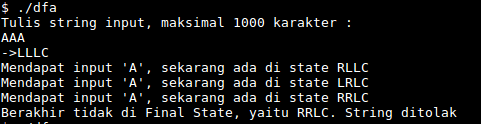
\includegraphics[width=350pt]{AAA.png}
\end{figure}

Lalu, program dites menggunakan masukan yang \textit{valid}, yaitu AAB. Hasilnya adalah :
\begin{figure}[h!]
  \centering
  \caption{Tes kedua, masukan \textit{valid}}.
  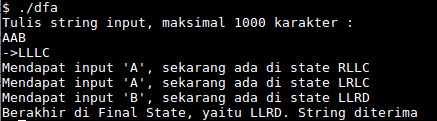
\includegraphics[width=350pt]{AAB.png}
\end{figure}

Dari kedua tes tersebut, didapat bahwa program melakukan simulasi \textit{state-state} yang dilalui dengan benar. Selain itu, program juga memberikan kesimpulan tentang diterima atau tidaknya sebuah masukan dengan benar.

\end{document}
